\documentclass[12pt]{report}
\usepackage[utf8]{inputenc}
\usepackage{tabularx} % extra features for tabular environment
\usepackage{amsmath,amssymb,amsthm}  % improve math presentation
\newcommand{\E}{\mathrm{E}}
\newcommand{\Var}{\mathrm{Var}}
\newcommand{\Cov}{\mathrm{Cov}}
\newcommand{\Cor}{\mathrm{Cor}}
\DeclareMathOperator*{\argmin}{argmin}
\DeclareMathOperator*{\argmax}{argmax}
\newcommand\norm[1]{\left\lVert#1\right\rVert}
\newcommand\myleqa{\mathrel{\overset{\makebox[0pt]{\mbox{\normalfont\tiny\sffamily (a)}}}{\leq}}}
\newcommand\myleqb{\mathrel{\overset{\makebox[0pt]{\mbox{\normalfont\tiny\sffamily (b)}}}{\leq}}}
\newcommand\myleqc{\mathrel{\overset{\makebox[0pt]{\mbox{\normalfont\tiny\sffamily (c)}}}{\leq}}}
\newcommand\myeqa{\mathrel{\overset{\makebox[0pt]{\mbox{\normalfont\tiny\sffamily (a)}}}{=}}}
\newcommand\myeqb{\mathrel{\overset{\makebox[0pt]{\mbox{\normalfont\tiny\sffamily (b)}}}{=}}}
\usepackage{graphicx} % takes care of graphic including machinery
\usepackage[margin=1in,letterpaper]{geometry} % decreases margins
\usepackage{cite} % takes care of citations
\usepackage[final]{hyperref} % adds hyper links inside the generated pdf file
\hypersetup{
	colorlinks=true,       % false: boxed links; true: colored links
	linkcolor=black,        % color of internal links
	citecolor=black,        % color of links to bibliography
	filecolor=magenta,     % color of file links
	urlcolor=blue         
}
\usepackage{setspace}
\doublespacing

\begin{document}

\title{
{
\includegraphics[width=0.7\columnwidth]{university.jpg}}\\
{Greedy Principal Flows}\\
{\large National University of Singapore}\\
}
\author{Sebastian Lie}
\date{05 March 2021}
\maketitle

\chapter*{Acknowledgements}
My 7 soft toys. And my desk lamp for being the light of my life.

\chapter*{Abstract}
Principal Flows are a great tool to use when we want to extend the 
notion of Principal Component analysis to multivariate datasets that 
we know lie on non-linear manifolds. 
We restrict this problem to constructing principal flows on hyperspheres. 
We use a different, easier method to obtain the principal flow 
that is even closer to its canonical PCA interpretation. 

\newpage
\tableofcontents
\newpage

\chapter{Introduction}

\section{Motivation}

With the advent of Big Data, using machine learning on multivariate datasets 
to solve problems from disparate fields has grown in popularity. Although 
most problems take the form of classification or regression problems 
Unsupervised learning has also grown in popularity, 
Principal Component Analysis being the most popular algorithm. 
However, if it is given data that lie on some manifold, or a non-linear space, 
PCA fails to achieve good results. 
This is why we want to use Principal flows: 
in essence they are a generalisation of PCA to manifolds. 
Furthermore, in keeping with the trends of the data science field, 
we want to use a popular language, python to construct these principal flows.

\newpage

\section{Notation}

We first define notation and some important concepts we will use later.

\begin{table}[h]
\begin{tabular}{|l|l|}
\hline
\textbf{Notation} & \textbf{Explanation}                                      \\ \hline
$\mathbb{R}^D$    & D dimensional space of real numbers.                      \\ \hline
\textbf{X}        & Data Matrix, D dimensions                                 \\ \hline
$D$                & The original dimension of the data matrix                 \\ \hline
$d$               & Dimension of lower dimensional data which X is reduced to \\ \hline
$\mathcal{M}^d$      & Denotes a connected and complete d-dimensional manifold
                   embedded in $\mathbb{R}^D$                                 \\ \hline
$p$               & Denotes a point on the manifold, $\mathcal{M}^d$.            \\ \hline
\textbf{v}        & Denotes a vector.                                         \\ \hline
$T_pM$            & Denotes the Tangent space of a point p on $\mathcal{M}^d$.   \\ \hline
\textbf{S}        & Denotes a Covariance matrix.                               \\ \hline
$\{x_1,...x_n\}$  & Denotes a collection of n data points.        \\ \hline
$\mathbf{1}$      & Denotes a vector of 1s.                                   \\ \hline
$\textbf{I}$      & Denotes the identity matrix.                               \\ \hline
$M^T$             & Denotes the transpose of a some matrix M.                 \\ \hline
\end{tabular}
\end{table}

\newpage

\section{Definitions}

First we define the notion of vector fields.

\subsection{Vector Fields}
A vector \textit{at point p}, $p \in \mathbb{R}^{D}$ is a pair 
$\textbf{v} = (p, v), \ v \in \mathbb{R}^{D}$, such that $\mathbf{v}$ 
is the vector $v$ translated so that its tail is at $p$ instead of the origin. 
All vector operations are defined such that the first item of the pair remains the same, 
and the second item is the result of the operation. 
The length and angle between 2 vectors are the same as normal vectors rooted in the origin.
\textbf{Definition:} A \textit{vector field} \textbf{X} on 
$U \subset \mathbb{R}^{n+1}$ is a function which assigns to each point
of U a vector at that point. Then
$$\textbf{X}(p) = (p, X(p))$$ for some function 
$X: U \longrightarrow \mathbb{R}^{n+1}$. Vector fields on 
$\mathbb{R}^{n+1}$ are often most easily described by 
specifying this associated function X.
A pictoral example of a vector field is below.
\begin{figure}[h]
    \begin{center}
        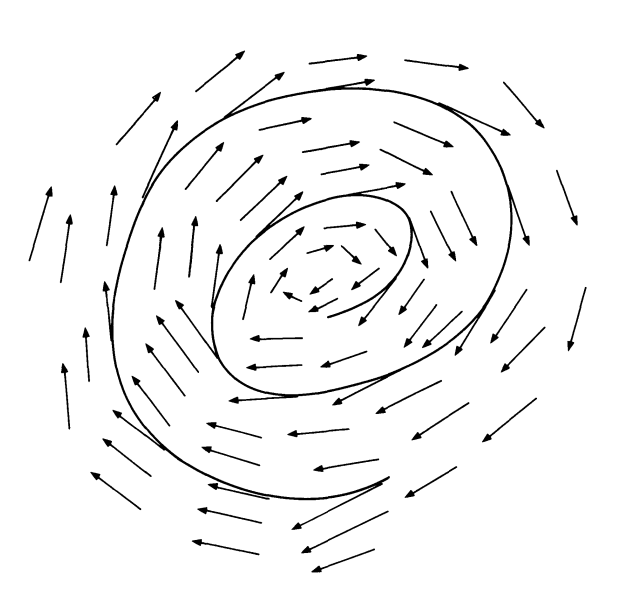
\includegraphics[scale=0.5]{fig2.5.PNG}
        \caption{An example of a vector field, $\mathbb{R}^3$}
        \label{fig:Graph 4}
    \end{center}
\end{figure}

\newpage

\subsection{Logarithm Maps}
\textbf{Logarithm Map:} For each $p \in M$, let
$$log_p(\textbf{v}):\mathcal{M}^d\longrightarrow T_pM$$
x is a vector
be the logarithm map. The log map is a function that projects a point $x_i$ 
on the manifold $\mathcal{M}^d$
onto the plane tangent to $\mathcal{M}^d$ at p, by producing a vector which indicates 
the direction in which p should move to obtain the projection of $x \in \mathcal{M}^d$ onto $T_pM$.\\
\\
\textbf{Exponential Map:} For each $p \in M$, let
$$exp_p(\textbf{v}): T_pM \longrightarrow \mathcal{M}^d$$
be the exponential map. Exponential maps are the inverse of the logarithm maps.
Given a point p, the exponential map w.r.t $\mathcal{M}^d$, a manifold, 
is a function that projects a point from the plane tangent to $\mathcal{M}^d$ at p onto $x$ 
on the manifold $\mathcal{M}^d$.\\

\subsection{Tangent Space}
Define graphically.
For a smooth function $f:U \longrightarrow \mathbb{R}$ 
where U is an open set $\in \mathbb{R}^D$, a vector u is said to be 
\textit{tangent to the level set} if
there is a well defined tangent space consisting of all velocity vectors 
at p of all parametrized curves in $f^{-1}(c)$ passing through p, 
and this tangent space is precisely the subspace consisting of 
all vectors orthogonal to $\nabla f(p)$. In the context of this report, 
the tangent space $T_pM$ is the hyperplane in which all vectors which are tangent to the point 
p on the $\mathcal{M}^d$ lie.
\begin{figure}[h]
    \begin{center}
        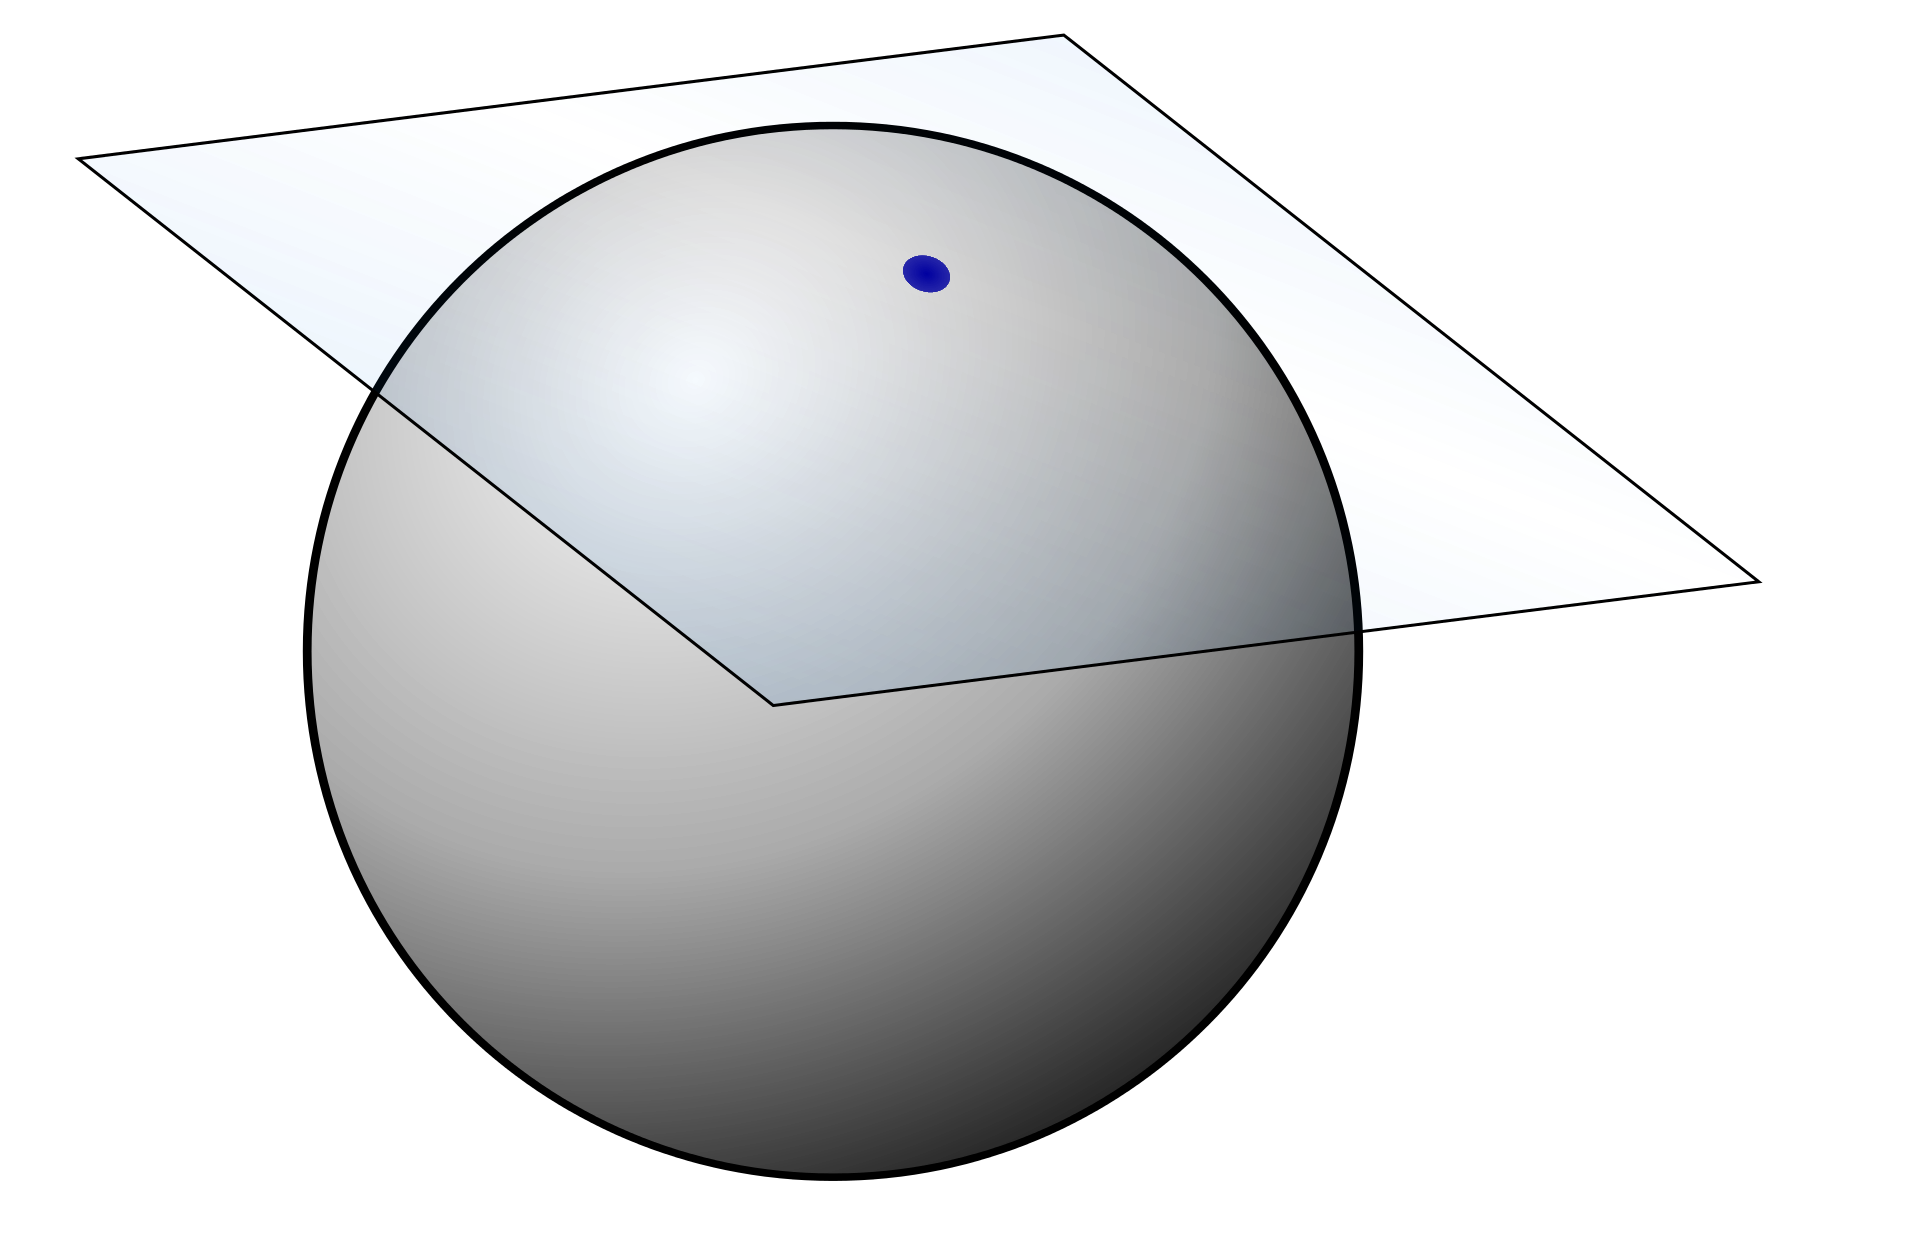
\includegraphics[scale=0.1]{tangent_space.png}
        \caption{Tangent Space of a sphere, $\mathbb{R}^3$}
        \label{fig:tanspace}
    \end{center}
\end{figure}

\subsection{Geodesics}

Geodesics are curves in d-surfaces or on d-dimensional manifolds
which play the same role as straight
lines in $\mathbb{R}^d$. They can be thought of as the "shortest path
between 2 points on the manifold, $\mathcal{M}^d$.\\
\\
\iffalse
or\\
\\
A geodesic on a d-dimensional manifold $\mathcal{M}^d \subset \mathbb{R}^D$ is a
parametrized curve $\alpha: I\longrightarrow M$ whose acceleration is everywhere
orthogonal to $\mathcal{M}^d$. Thus a geodesic is a curve in S which always goes" straight ahead" in
the surface,  Its acceleration serves only to keep it in the surface. It has no
component of acceleration tangent to the surface.\\
\fi
The Euclidean distance between 2 points $p, q$ 
is defined as $\norm{p-q}$, or the 2-norm of the vector $p-q$.
Geodesic distance extends this concept of Euclidean, straight line distance
in the Euclidean space to Manifolds. 


\subsection{Eigenvalues and Eigenvectors}
Now we define eigenvalues and eigenvectors.
\textbf{Definition}: Let $\textbf{A} \in \mathbb{R}^{n \times n}$. 
Then a non-zero vector \textbf{v} is an eigenvector of \textbf{A} 
if there exists some scalar $\lambda$ such that $\textbf{A}\textbf{v} = \lambda \textbf{v}$. 
Then $\lambda$ is known as the eigenvalue corresponding to vector \textbf{v}.\\
\\
Here we also note that for any 2 eigenvectors $v_i$ and $v_j$, $i \neq j$, $v_i \cdot v_j = 0$, 
or any 2 eigenvectors are orthogonal to each other, and that $v_i \cdot v_i = 1$.

\subsection{Diagonalisation}

We say that a matrix is diagonalisable if $\exists \textbf{V}$, 
an orthonormal matrix such that the rows of \textbf{V} 
are the eigenvectors of \textbf{C},  and a diagonal matrix 
$\textbf{E}$ whose diagonal values are the eigenvalues of \textbf{C}.
In the context of this report, we only consider 
symmetric matrices given by $\textbf{C} \in \mathbb{R}^{D \times D}$, 
which are always diagonalisable.
$$\textbf{C} = \textbf{V}\textbf{E}\textbf{V}^T$$

\chapter{Literature Review}

\section{Linear Dimension Reduction}

\subsection{Principal Component Analysis}

\textbf{Principal Component analysis} is a linear dimension reduction method 
which tries to obtain a lower-dimensional representation of the data 
that retains as much variation as possible present in the data set. 
PCA does this by constructing principal components (PCs) 
which are linear combinations of the centered original variables. 
Note that centering each column is the same as finding the "mean" 
observation and subtracting that from every observation: $x_i - \bar{x}$, 
since $\bar{x}$ contains the means of every column.
These PCs are uncorrelated (orthogonal) and ordered in descending order 
by the amount of variation retained. 
Then, reducing some high-dimensional data of dimension $D$ to a lower dimensional $d$ 
is simply a matter of computing the first $d$ principal components.\\
\textbf{Algorithm}
\begin{itemize}
    \item 1. First we center the data matrix, \textbf{X}, by centering each column of \textbf{X}.
    \item 2. Next we compute the covariance matrix of the centered data matrix.
    \item 3. Now we diagonalise the covariance matrix and take the first d eigenvectors. 
    Let these d eigenvectors be the columns of a matrix $\textbf{V}_d$.
    \item 4. Multiply \textbf{X} by $\textbf{V}_d$ to obtain the d principal components.
\end{itemize}

\subsection{Classical MDS, Euclidean Distance}

\textbf{Multidimensional Scaling} is a linear dimensionality reduction method. 
Its main aim is to take some high dimensional data, \textbf{X} 
and find some low dimensional points so as to minimize the discrepancy 
between the pairwise distances in the original space and the pairwise distances 
in the lower-dimensional space. \\
Let a squared dissimilarity matrix between n points be 
$\textbf{M} \in \mathbb{R}^{n \times n}$, 
let the matrix of coordinates be denoted by 
$\textbf{X} \in \mathbb{R}^{n \times D}$, 
and let $\textbf{B} = \textbf{X}\textbf{X}'$. 
Since dissimilarities do not change under translations, 
we assume that \textbf{X} has column means equal to 0. 
MDS seeks to find a lower dimensional representation 
$\textbf{X}_{(d)} \in \mathbb{R}^{n \times d}$.\\
Algorithm: from 2005 Book Modern Multidimensional Scaling, pg 262
\begin{itemize}
    \item 1. Compute or obtain the dissimilarity matrix, \textbf{D}.
    \item 2. Let \textbf{J} be the centering matrix: $\textbf{J} = \textbf{I} - n^{-1}\mathbf{1}\mathbf{1}'$. Compute $\textbf{B} = -\frac{1}{2}\textbf{J}\textbf{D}\textbf{J}$.
    \item 3. Then, compute the eigendecomposition of \textbf{B}: $\textbf{B} = \textbf{V}\mathbf{\Lambda}\textbf{V}'$. 
    \item 4. Then $\textbf{X} = \mathbf{\Lambda}^{1/2}\textbf{V}'$ 
    and for a d-dimensional representation of 
    \textbf{X}: $\textbf{X}_{(d)}$, $\textbf{X}_{(d)} = \mathbf{\Lambda}^{1/2}_d\textbf{V'}_d$, 
    where $\mathbf{\Lambda}^{1/2}_d$ is the first $d \times d$ submatrix of $\Lambda$,
     and $\textbf{V'}_p$ is the first d columns of \textbf{V}', 
     i.e the first d eigenvectors and their corresponding eigenvalues.
\end{itemize}
Note that using Euclidean distances, the result of MDS is the same as PCA.
Advantages of MDS over PCA: If we have $n << p$, then MDS is likely to be more efficient, 
since MDS finds eigenvectors of a $n \times n$ matrix and a $p \times p$ matrix respectively. 
(From 2002 book on Principal Component Analysis)
MDS simple to implement, and their optimizations 
do not involve local minima despite their inherent limitations as linear methods.

\section{Non-Linear Dimension Reduction}

Non-linear dimensionality reduction methods are particularly useful 
when the multivariate data we obtain is sampled from a smooth non-linear manifold $\mathcal{M}^d$, 
e.g a manifold in an S-shape, obtains better estimates than linear methods like PCA and MDS, 
which implicitly assume that the data is sampled from a linear space. 
Certain data sets contain essential nonlinear structures that are invisible to PCA and MDS.

\newpage

\subsection{Principal Geodesic Analysis}

Principal Geodesic Analysis(PGA) is a generalization of 
principal component analysis to connected, 
complete manifolds. The main aim of PGA is to be able to 
describe the variability of some data lying on some manifold $\mathcal{M}$. 
More formally, the goal is to find a sequence of lower-dimensional subspaces, 
which on manifolds are nested geodesic submanifolds 
that maximize the projected variance of the data. 
These submanifolds are called the principal geodesic submanifolds, 
which are analogous to linear subspaces for PCA.\\
Let $T_pM$ be the tangent space of $\mathcal{M}$ at the intrinsic mean $p$ of the $x_i$. 
The intrinsic mean of some data \textbf{X} lying on some manifold is obtained 
by first setting the initial mean to a random data point, 
then iteratively obtaining a better estimation of the intrinsic mean 
by computing the average of the vectors obtained using the log map at 
the current mean on all data points, then taking the next estimate of the 
intrinsic mean as the projection of that average using the exponential map 
at the current estimate.\\
Let $U \subset T_pM$ be a neighbourhood of 0 in which our data, 
$\{x_1,...x_n\}$ lies, such that projection is well defined 
for all geodesic submanifolds of $exp_p(U)$.These principal geodesic submanifolds 
are obtained by by first constructing an orthonormal basis of tangent vectors 
$v_1,...,v_d \in T_pM$ that span the tangent space. 
These vectors are then used to form the principal geodesic subspaces 
$H_k$ where $H_k = exp_p(V_k)$, and $V_k$ is intersection of the 
subspace spanned by vectors $1..k$ and $U$.
subspace $V_k = span(\{v_1,...,v_k\})\bigcap U$.\\
\textbf{Algorithm}:
\begin{itemize}
    \item 1. Obtain the intrinsic mean, $p \in \mathcal{M}^d$ of $\{x_1,..x_n\}$.
    \item 2. Calculate the vectors $u_i = log_p(x_i)$.
    \item 3. Calculate the covariance matrix $\textbf{S} = \frac{1}{n} \sum^n_{i=1} u_iu_i^T$.
    \item 4. Diagonalise the covariance matrix to obtain $\{v_k, \lambda_k\}$ 
    the eigenvectors and eigenvalues respectively, 
    which represent the principal directions in the tangent space $T_pM$ and the variances.
\end{itemize}

\newpage

\subsection{Locally Linear Embedding}

\textbf{Locally Linear Embedding}
\\
The main idea of LLE is to construct a neighbourhood preserving mapping 
of the original points of dimension $D$ to the reconstructed points of dimension $d$. 
We assume that for some data $\textbf{X} \in \mathbb{R}^{D}$, 
the data lie on or near a smooth manifold of dimensionality $d << D$. 
Locally, LLE assumes the embedding is linear, and thus for each data point $p \in \mathbb{R}^D$, 
we aim to use a linear combination of its K nearest neighbours to reconstruct a lower-dimensional $p \in \mathbb{R}^d$. 
LLE does this by first learning some reconstruction weights from the D-dimensional data: $\textbf{W}$ 
where $\textbf{W}_{ij}$ represents the contribution of the j-th data point in reconstructing the i-th one. 
These weights obey an important symmetry: for any particular data point, 
they are invariant to rotations, rescalings, and translations of that data point and its neighbors.
They thus reflect intrinsic geometric properties of the data that are invariant to exactly such transformations,
and therefore, we expect their characterization of local geometry in the 
original data space to be equally valid for local patches on the manifold.
This is what motivates $\textbf{W}_{ij}$ to be used to reconstruct
the embedded manifold coordinates in $d$ dimensions. 
At the end of LLE, each  D-dimensional observation $\textbf{X}_i$ 
is mapped to a low dimensional vector $\textbf{Y}_i$ 
representing global internal coordinates on the manifold.\\
\textbf{LLE Algorithm:}
\begin{itemize}
    \item 1. Compute the K nearest Neighbors of each original data point 
    $\textbf{X}_i$, where K is a hyperparameter.
    \item 2. Compute the weights $\textbf{W}_{ij}$ that best 
    reconstruct each data point from it's neighbours 
    minimizing the \textbf{Reconstruction Error} below by constrained linear fits.
$$\varepsilon (\textbf{W}) = \sum_i|\textbf{X}_i - \sum_j \textbf{W}_{ij} \textbf{X}_j|^2$$
    \item 3. Compute the vectors $\textbf{Y}_i$ best reconstructed by the weights $\textbf{W}_{ij}$ 
    by minimising the embedding cost function: 
    $$\Phi(\textbf{Y}) = \sum_i |\textbf{Y}_i - \sum_j \textbf{W}_{ij}\textbf{Y}_j|^2$$
    This is minimised by solving a sparse $N \times N$ 
    eigenvector problem whose bottom d non-zero eigenvectors provide
    an ordered set of orthogonal coordinates centered on the origin.
\end{itemize}

\newpage

\subsection{Isomap}

Isomap is an extension of MDS to manifolds in which embeddings 
are optimized to preserve geodesic distances between pairs of data points.
It combines the major algorithmic features of PCA and MDS
 — computational efficiency, global optimality, 
 and asymptotic convergence guarantees — 
 with the flexibility to learn a broad class of nonlinear manifolds.
 Isomap achieves this by estimating the geodesic distance between data points, 
 given only input-space distances, e.g euclidean distance between points.\\
\\
This relies on the fact that for neighboring points, 
input-space distance provides a good approximation to geodesic distance. 
For faraway points, Isomap approximates geodesic distance 
by adding up a sequence of “short hops” between neighboring points, 
computed efficiently by finding shortest paths in a graph with edges 
connecting neighboring data points.  
This approximation relies on the proof that for a 
sufficiently high density of data points, 
we can always choose a neighborhood size (e or K) large enough 
that the graph will (with high probability) have a path not much longer 
than the true geodesic, but small enough to prevent edges 
that “short circuit” the true geometry of the manifold.\\
\textbf{Isomap Algorithm}:
\begin{itemize}
    \item 1. Construct neighbourhood graph $G$: 
    First, we need to compute the distances between points: 
    for any node i and j, connect the 2 nodes if 
    $d(i,j) < \epsilon$ or if j is one of the k-nearest neighbours of i.
    \item 2. Compute all-pairs shortest paths on $G$. 
    There are many algorithms to do this, but we use the Floyd-Warshall algorithm.
    \item 3. Construct d-dimensional embedding, using MDS.
\end{itemize}

\chapter{Greedy Principal Flows}

\section{Problem Statement}

The main objective for greedy principal flows was to quantify or describe 
multivariate data on the manifold: we cannot simply fit a line, 
as this is not Euclidean space.
Instead, we want some curve or path such that, 
locally, and globally, it follows the path of maximal variation of the data. 
The first principal flow can be thought of as 
the manifold extension of the 1st principal component in euclidean space.
This has already been done in \cite{principalflow}, where the principal flows 
were constructed by solving a problem in variational calculus.
Here, we focus on constructing the principal flow using a novel, 
simpler to implement approach: a greedy algorithm.

\section{An explanation of the algorithm}

Throughout we will assume that \textbf{X} lies on the hypersphere. 
To find our principal flow, we first need a starting point. Since our principal flow 
follows the path of maximal variation of our data, 
we know it should pass through the centroid of the data. 
Thus, we first aim to find or estimate this centroid.
Although there are many ways of doing this, we opt to make use of the fact that 
the first principal component passes through the centroid of the data. Thus, if we 
iteratively project all the data onto the tangent space of the hypersphere, 
find the 1st principal direction, move in that direction, 
and find the projected point on the hypersphere, we will eventually converge on the 
centroid.
\\
\textbf{Centroid Algorithm}:
\begin{itemize}
    \item 1. Let $p = x_i$, a random data point.
    \item 2. Compute $log_p(x_i)$ for all $x_i$, and let these vectors be the rows of the matrix $\bar{\textbf{X}}$.
    \item 3. Calculate the covariance matrix of $\bar{\textbf{X}}$.
    \item 4. Diagonalise the matrix, then save the eigenvector corresponding to the largest eigenvector, $\textbf{v}_1$.
    \item 5. Move in the direction of $\textbf{v}_1$ a step size of $\epsilon$, $p' = p + \epsilon \textbf{v}_1$.
    \item 6. Let $p = exp_p(p')$.
\end{itemize}
Then we start from that centroid, and build our principal flow from there.
Our aim is to find the path of maximal variation of the data.\\
\textbf{Problem}:\\
What if our data stretches all around the hypersphere? How do we deal with projecting
data through the sphere?\\
Instead of taking all data into consideration, we choose a small neighborhood around
our centroid, whose size is controlled by h. This neighbourhood is determined 
by some kernel function: either binary or gaussian. The binary kernel 
includes points in some neighbourhood and excludes points outside,
while the gaussian kernel weights nearer points in some neighbourhood 
much more than those outside the neighbourhood. Thus, we
project the data within some neighbourhood $\textbf{X}_h$ onto the tangent space 
at the centroid, p: $T_pM$. We use the logarithm map, $log_p$ to do this. Then the path of maximal variation 
in this neighbourhood of points is the first principal direction of this data from PCA. 
This direction is obtained by diagonalising the covariance matrix of the data on this tangent
space. \\
\textbf{Problem}:\\
This direction clearly is not accurate if we only move in this direction,
since it will eventually lead us out of the surface of the hypersphere, and even on the 
hypersphere, the neighbourhood of points may differ, and change the direction 
of the path of maximal variation.\\
Thus, instead of only using this direction, we move infinitesimally in this first direction,
then carry out the same procedure again. Thus we iteratively find the "local"
direction of maximal variation, move in that direction, and re-compute the next direction
of maximal variation. We continue doing this until we have obtained a flow through the
entire data set.\\
This does indeed follow the framework that isomap and LLE abide by
as well: that obtaining the best option locally becomes the best option globally as well. 
This is exactly the idea of this Greedy Principal flow algorithm. 

\section{Algorithm Steps}
Defn: The Principal Flow of the dataset is basically an integral curve 
that is always tangent to the direction of 'maximal variation' at any given point 
it contains.
\begin{itemize}
    \item We assume the underlying structure of the data is a hypersphere.
    Starting from the centroid of the data set (user defined or calculated below), we apply the following procedure: 
    \item 1. Project the data residing on the hypersphere onto the hyperplane
    tangent to the centroid of the data (p). We use the log map of p, 
    obtaining a matrix of vectors on the tangent plane that point from p
    to the projected points. These are the plane vectors.

    \item 2. Compute the largest principal component of the points 
    using the plane vectors, applying weights as necessary via the kernel function provided.

    \item 3. The largest principal component is the new directions 
    that the principal flow moves in. We determine it's sign by making sure
     it is moving in the same direction as the previous principal direction.

    \item 4. We take a small step in each direction on the plane,
    then project it back to the hypersphere.

    \item 5. We do 1-4 for the point on the opposite end of the growing principal flow.

    \item 6. Store both points. 
    
    \item 7. Repeat 1-6 until max\_iter is reached.
\end{itemize}

\chapter{Greedy Principal Boundary}

In the section above, we have already seen the principal flow.
Now we extend the idea of Principal flows to attempt to find some boundary of the data.
Let us imagine that the data is contained on some ellipse of the manifold
$\mathcal{M}$. Then our aim is to find some boundary around this ellipse. We proceed 
similarly to the principal flow, except that we also take the 1st and 2nd largest eigenvector
and eigenvalues. Here in this context

\begin{itemize}
    \item We assume the underlying structure of the data is a hypersphere.
    Starting from the centroid of the data set (user defined or calculated below) we
    iteratively do the steps below:

    \item 1. Project the data residing on the hypersphere onto the hyperplane
    tangent to the centroid of the data (p). We use the log map of p, 
    obtaining a matrix of vectors on the tangent plane that point from p
    to the projected points. These are the plane vectors.

    \item 2. Compute the 1st and 2nd largest eigenvector and their associated
    eigenvalues of the covariance matrix of the points using the plane vectors, 
    applying weights as necessary via the kernel function provided.

    \item 3. Use the eigenvalues obtained to calculate the radius of the
    \item ellipse of the data. Then we move a distance of this radius, in the direction
    \item indicated by the 2nd largest eigenvector.

    \item 4. We take a small step in each direction on the plane,
    then project it back to the hypersphere.

    \item 5. We do 1-4 for the point on the opposite end of the growing principal flow.

    \item 6. Store both points. 
    
    \item 7. Repeat 1-6 until max\_iter is reached.
\end{itemize}

\section{Algorithm}

\chapter{Applications}
Writing the algorithm is meaningless without testing that it also functions 
as we want it to. First we start with simple applications on toy data to confirm that 
our algorithm works as intended, then we apply it on some real world data to show
how the principal flow can be used there as well.

\section{Toy Data}

\subsection{Without Noise}

As a sanity check or proof of concept of our principal flow, 
we first want to test our algorithm on some toy data that we know 
lies on the 3-dimensional unit sphere. This will help us visualise the flow created
and determine if it follows the pattern of the data, 
and thus act as a proof of concept of
our algorithm. We generate some data artificially.


\begin{figure}[h]
    \begin{center}
        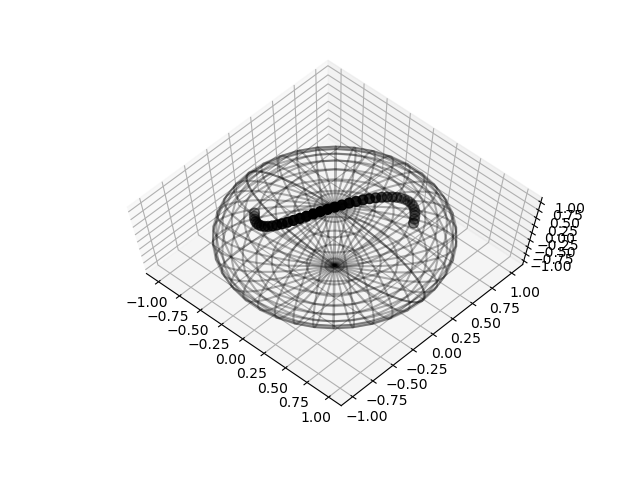
\includegraphics[]{Data_13.png}
        \caption{Toy data 13, $\mathbb{R}^3$}
        \label{fig:toydata}
    \end{center}
\end{figure}

\newpage

For example, this dataset is created by setting the first coordinate of the 
i-th point to $\frac{i-n/2}{n}$, the second to $sin(4*1st)/2$, and the third to 
$\sqrt{1-(1st)^2 - (2nd)^2}$, where n is the number of points we want to generate.\\
Now that we have seen the Toy Data, let us apply the Principal Flow 
algorithm to the data above.

\begin{figure}[h]
    \begin{center}
        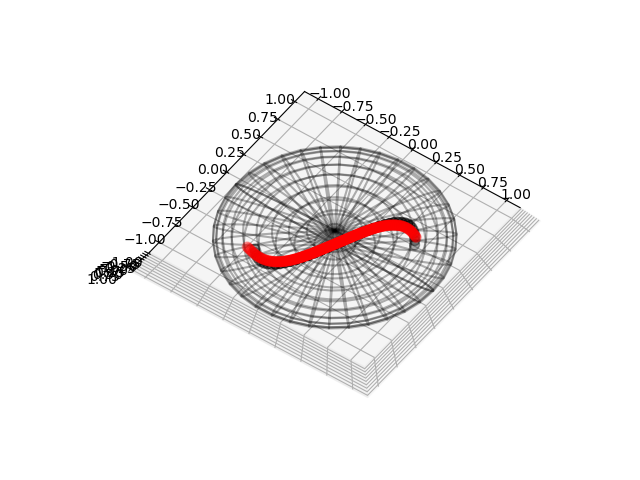
\includegraphics[]{single_flow_13.png}
        \caption{Principal Flow on Toy Data, $\mathbb{R}^3$}
        \label{fig:pflowtoy}
    \end{center}
\end{figure}

This 3D plot shows the original data in black, and the principal flow in 
\textcolor{red}{red}.
With some tuning of h, the size of the neighbourhood, we can see that we have constructed
a principal flow that follows the original data almost
exactly, reconstructing an S with some slight differences at the curves of the s-shape of
the original data.
We have now seen that proof that our principal flow algorithm works:
it is able to accurately reconstruct the toy data, 
the s curve on the sphere.

\subsection{With Noise}

Next, gaussian noise was added to the S-shaped data on the sphere to create a noisy dataset.
Then we fitted a principal flow to this noisy data.

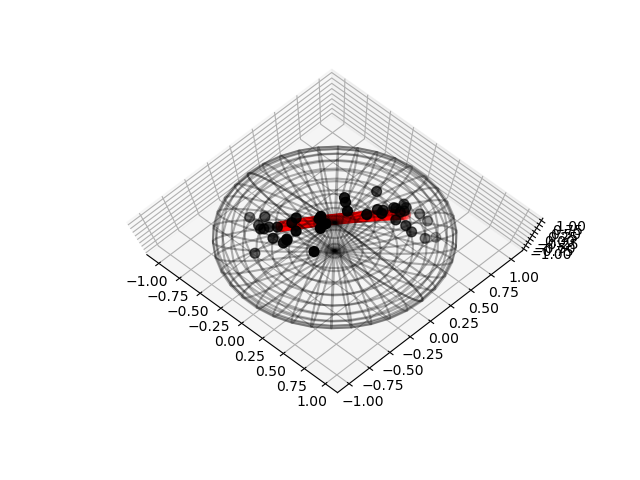
\includegraphics[]{noisy_13.png}

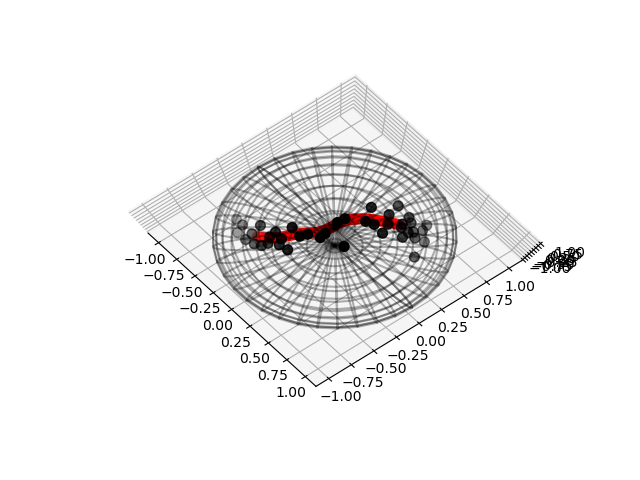
\includegraphics[]{noisy_13_gaussian.png}

We can see that the principal flow obtained seems to follow the new pattern 
of variation in the data: from the more dense cloud of points on the left, to the curve of
the points in the center to the other dense cloud of points on the right.

\subsection{Boundary Flow with Noise}


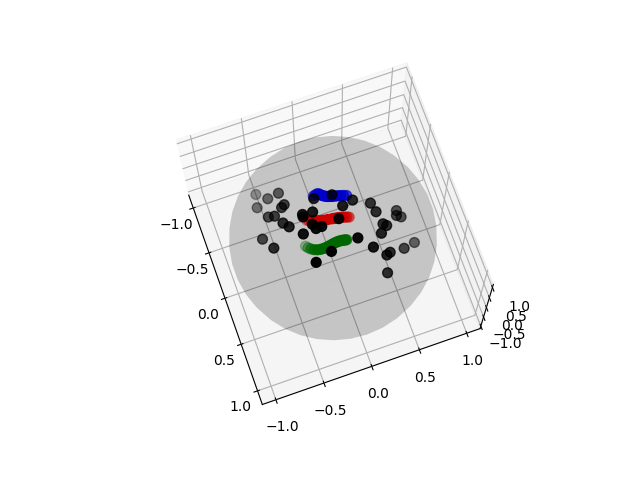
\includegraphics[]{noisy_boundary_flow13.png}

\section{Real World Data}

\subsection{MNIST}

\begin{figure}[h]
    \begin{center}
        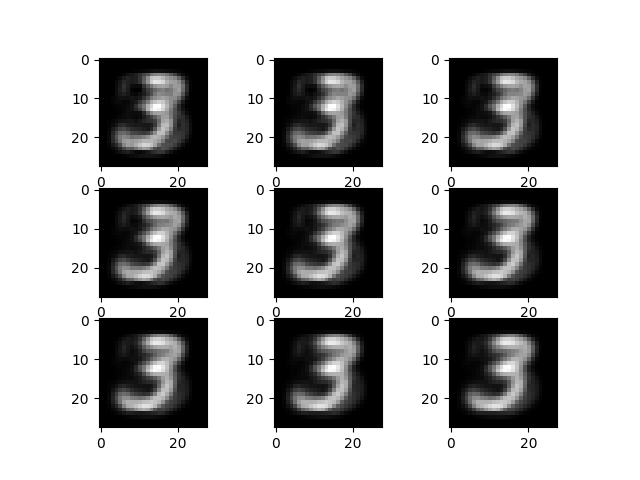
\includegraphics[]{mnist1.png}
        \caption{MNIST Flow, part 1}
        \label{fig:pflowtoy}
    \end{center}
\end{figure}



\begin{figure}[h]
    \begin{center}
        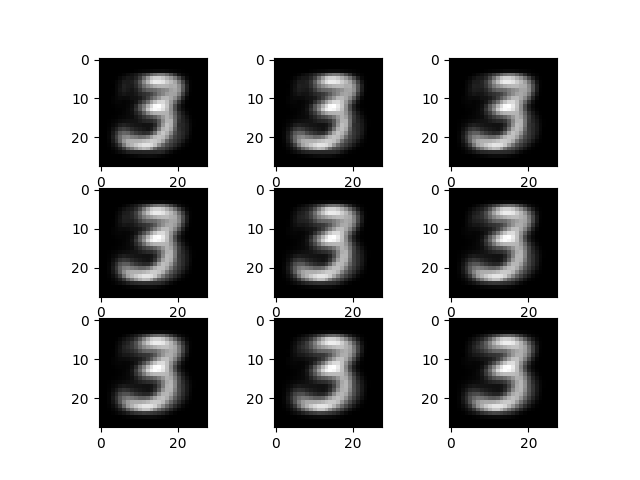
\includegraphics[]{mnist2.png}
        \caption{MNIST Flow, part 2}
        \label{fig:pflowtoy}
    \end{center}
\end{figure}


\begin{figure}[h]
    \begin{center}
        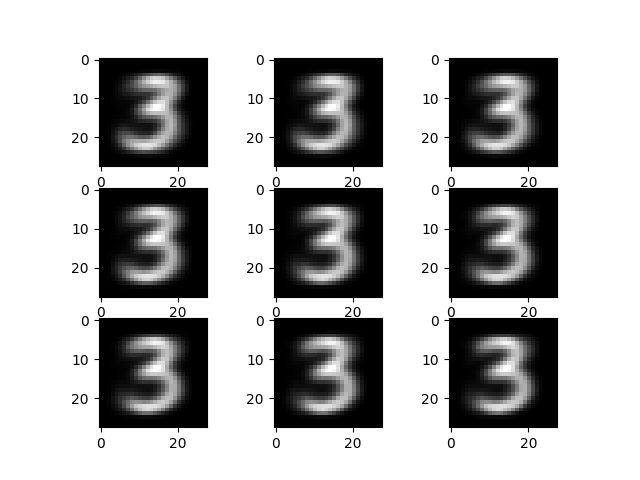
\includegraphics[]{mnist3.png}
        \caption{MNIST Flow, part 3}
        \label{fig:pflowtoy}
    \end{center}
\end{figure}


\begin{figure}[h]
    \begin{center}
        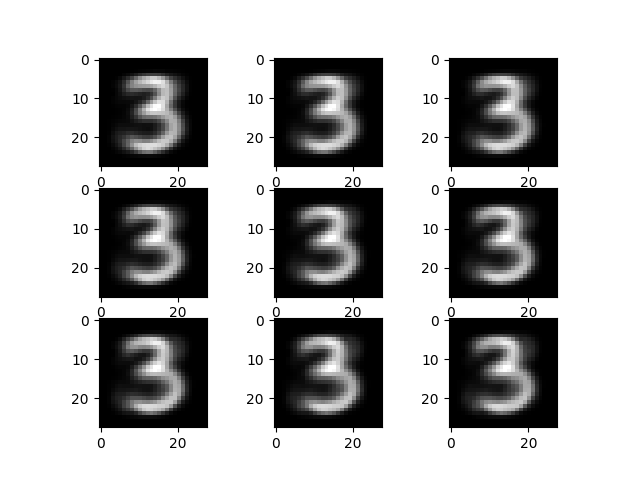
\includegraphics[]{mnist4.png}
        \caption{MNIST Flow, part 4}       
        \label{fig:pflowtoy}
    \end{center}
\end{figure}

\subsection{Fashion MNIST}



\subsection{Olivetti faces}


\chapter*{Future Directions}

What open questions can we investigate further?


\chapter{References}
\begin{thebibliography}{9}

\bibitem{mds}
Ingwer Borg and Patrick J.F. Groenen (2005) \textit{Modern Multidimensional Scaling}, Springer.

\bibitem{pga}
P. Thomas Fletcher, Conglin Lu, Stephen M. Pizer and Sarang Joshi \textit{Principal Geodesic Analysis for the Study of
Nonlinear Statistics of Shape}

\bibitem{isomap}

\bibitem{principalflow}
Victor M. Panaretos, Tung Pham and Zhigang Yao (2014) Principal Flows, Journal of the American Statistical
Association, 109:505, 424-436, DOI: 10.1080/01621459.2013.849199


\end{thebibliography}

\end{document}